\documentclass[letterpaper, 10pt, conference]{ieeeconf}
\usepackage{times}


\IEEEoverridecommandlockouts 
\overrideIEEEmargins


\usepackage{cite}
\usepackage{graphicx}     
\usepackage{amssymb,amsmath}
\usepackage{algorithm}
\usepackage[noend]{algorithmic}
\usepackage{flushend}
\renewcommand{\thefootnote}{\fnsymbol{footnote}}

\usepackage{color}

\newcommand{\Acronym}[1]{\ensuremath{{\small{\texttt{#1}}}}}
\newcommand{\Symbol}[1]{\ensuremath{\mathcal{#1}}}
\newcommand{\Function}[1]{\ensuremath{{\small \textsc{#1}}}}
\newcommand{\Constant}[1]{\ensuremath{\small{\texttt{#1}}}}
\newcommand{\Var}[1]{\ensuremath{{\small{\textsl{#1}}}}}
\newcommand{\False}{\Constant{false}}
\newcommand{\True}{\Constant{true}}
\newcommand{\Null}{\Constant{null}}
\newcommand{\Name}{\Acronym{dCRoPS}}
\newcommand{\Revision}[1]{\textcolor{red}{#1}}
\newcommand{\R}{\ensuremath{\mathbb{R}}}
\newcommand{\Traj}{\ensuremath{\zeta}}
\newcommand{\Tree}{\Symbol{T}}

\setlength{\abovedisplayskip}{1pt}
\setlength{\belowdisplayskip}{1pt}

\begin{document}

\title{Path Planning for Swarms in Dynamic Environments by\\ Combining Probabilistic Roadmaps and
  Potential Fields}


\author{
Alex Wallar \and Christopher Choi \and Erion Plaku
\thanks{A. Wallar and C. Choi are with the School of Computer Science,
  University of St Andrews, Fife KY16 9AJ, Scotland, UK. E. Plaku is with the
  Dept. of Electrical Engineering and Computer Science, Catholic
  University of America, Washington DC 20064 USA.
}}

\maketitle
\begin{abstract}
This paper presents a path-planning approach to enable a swarm of
robots move to a goal region while avoiding collisions with static and
dynamic obstacles.  To provide scalability and account for the
complexity of the interactions in the swarm, the proposed approach
combines probabilistic roadmaps with potential fields.  The underlying
idea is to provide the swarm with a series of intermediate goals which
are obtained by constructing and searching a roadmap of likely
collision-free pathways. As the swarm moves from one intermediate goal
to the next, it relies on potential fields to quickly react and avoid
collisions with static and dynamic obstacles. Potential fields are
also used to ensure that the swarm moves in cohesion. When the swarm
deviates or is unable to reach the planned intermediate goals due to
interferences from dynamic obstacles, the roadmap is searched again to
provide alternative pathways. Experiments conducted in simulation
demonstrate the efficiency and scalability of the approach.
\end{abstract}


\section{Introduction}
\label{sec:Intro}

Emerging applications of swarm robotics in exploration, monitoring,
inspection, and search-and-rescue missions require the swarm to be
able to move in cohesion to a goal destination while avoding
collisions with obstacles.  To provide scalability and account for the
complexity of the interactions in the swarm, this paper builds upon
prior work which combined probabilistic roadmaps with potential
fields. While prior work was limited to static obstacles, the proposed
approach can efficiently guide the swarm to the goal even in the
presence of dynamic obstacles. The underlying idea is to provide the
swarm with a series of intermediate goals which are obtained by
constructing and searching a roadmap of likely collision-free
pathways. As the swarm moves from one intermediate goal to the next,
it relies on potential fields to quickly react and avoid collisions
with static and dynamic obstacles. Potential fields are also used to
ensure that the swarm moves in cohesion. When the swarm deviates or is
unable to reach the planned intermediate goals due to interferences
from dynamic obstacles, the roadmap is searched again to provide
alternative pathways. Experiments conducted in simulation demonstrate
the efficiency and scalability of the approach.



Swarm robotics seeks to enable a large number of robots to accomplish
complex tasks via simple interactions with one another and the
environment \cite{reynolds1987flocks}.  Swarm robotics draws
inspiration from social insects, such as ants and bees, where
intelligent group behaviors emerge from simple interactions among the
individuals. Such framework provides a level of scalability and
robustness that is difficult to achieve with centralized
approaches. As research progresses, applications of swarm robotics are
emerging in exploration, mapping,
monitoring, inspection, and search-and-rescue missions, as surveyed in
\cite{swarm,swarmReview12}.

In many of these applications, the swarm needs to move in
cohesion to a goal destination while avoiding collisions with
obstacles and among the robots in the swarm. This path-planning
problem presents significant challenges. As path
planning is PSPACE-complete, exact algorithms, which always find a
solution if it exists and report no solution otherwise, are difficult
to implement and are limited in practicality to low-dimensional
systems due to the exponential dependency on the problem dimension
\cite{Rei79,Can88,SchSha88}.
As a result, research has focused on alternative approaches that do
not determine the existence of a solution but seek instead
to achieve efficiency and scalability in increasingly complex
settings.


A common approach in path planning for robotic swarms is to impose
artificial potential functions (APFs) that seek to push the swarm away
from the obstacles and toward the goal
\cite{Khatib86,reif1999social,book:SwarmsAPFs,tanner2005formation}. APFs
provide scalability as the addition of new robots to the swarm
generally requires only computation of repulsive forces from
obstacles, attractive forces from the goal, and forces resulting from
the limited interactions with neighboring robots.  However, an
inherent challenge with APFs is the tendency to get stuck in local
minima especially when planning paths for large swarms moving in
cluttered environments and through narrow passages.  APFs that avoid
local minima exist in limited cases, e.g., a point robot in a
generalized sphere world \cite{RK92}, but not for general path
planning for swarms.
 
Alternative approaches aim to avoid local minima by relying on
probabilistic roadmaps (PRMs) \cite{PRM}. PRMs capture the
connectivity of the configuration space via a roadmap obtained by
sampling collision-free configurations and connecting neighboring
configurations with collision-free paths. A configuration generally
specifies the placement of each robot in the swarm and a path between
two configurations is typically obtained by interpolation.  A
collision-free path from an initial to a goal configuration is then
obtained by performing graph search on the roadmap.  Starting with the
original PRM \cite{PRM} and continuing over the years, PRMs have had
great success in solving challenging problems
\cite{TogglePRM,UOBPRM,PlakuTRO05,HSUBridge,GaussianPRM,manocha12}.
The work in \cite{PRMapf1,PRMapf2} use APFs to increase PRM sampling
near obstacles to facilitate connections through narrow passages.  The
work in \cite{LienSwarming,LienSwarmingRules,LienShepherding} uses PRM
to enable robotic swarms achieve different behaviors such as homing,
coverage, goal searching, and shepherding. The roadmap, however, is
built over the high-dimensional configuration space, which
considerably increases the computational cost. The work in
\cite{KostasSwarm} uses multi-level PRMs in combination with Bezier
curves to guide a multi-robot system to a desired destination while
maintaining a specific formation. The approach has been applied only
to a small number of robots and requires considerable precomputation
to build the multi-level PRMs.


Even though significant progress has been made, scalability still
remains problematic in PRMs \cite{book:MP,book:LaValle}. As the number
of robots increases, it becomes difficult to sample collision-free
configurations and generate collision-free paths that connect
neighboring configurations. Moreover, significantly larger roadmaps
are needed to capture the connectivity of the configuration space.  As
a result, efficiency of PRMs starts deteriorating as the number of
robots is increased. These issues become even more problematic when
considering robotic swarms since PRMs do not have a mechanism to
ensure that the robots move in cohesion as a swarm rather than as
individual entities.


To improve the efficiency of path planning for robotic swarms, this
paper develops a novel approach, named $\Name$ (\texttt{C}ombined
\texttt{Ro}admaps and \texttt{P}otentials for \texttt{S}warms), which
combines APFs with PRMs.  While $\Name$ draws from PRM the underlying
idea of using a roadmap, it does not suffer from scalability issues as
the roadmap is constructed over the two-dimensional workspace instead
of the high-dimensional configuration space of the swarm. Moreover,
$\Name$ does not use the roadmap to plan the entire path of the swarm,
but rather to generate a series of intermediate goals that serve as
attractive potentials to guide the swarm toward the desired
destination. $\Name$ then relies on APFs to enable the robots move in
cohesion as a swarm from one intermediate goal to the other while
avoiding collisions. This combination of PRMs with APFs is crucial to
the efficiency and scalability of $\Name$. Experimental results in
simulation with increasingly large swarms moving in complex
environments containing numerous obstacles and narrow passages provide
promising validation.


\section{Method}
\label{sec:Method}

The swarm motions are governed by the following criteria:
\begin{enumerate}
\item There is long range attraction to intermediate goals and final destination. 
\item Robots are repulsed from obstacles.
\item Robots move as a swarm while keeping some separation from one another.
\item A robot's heading is influenced by the headings of its neighbors.
\end{enumerate}

In order to guide the swarm to the final destination, a global path planner is
used. A PRM is used to determine the shortest weighted path from the initial
configuration to the final configuration. The roadmap for the PRM is
constructed by taking by sampling collision free points and connecting
collision free neighboring edges. The result of the PRM sampling is a graph
that represents the connectivity of the configuration space. The vertices in
the roadmap are weighted according to an estimate of how well the swarm will
perform in that area of the environment. The edges are weighted according to
the distance from the two vertices on a given edge. With these weights, the
shortest path in the graph is computed using Dijkstra's algorithm. With the set
of vertices that lie on the shortest path, we are able to give the boids a set
of intermediate goals. By traversing the intermediate goals, the swarm will
effectively reach the final destination. An attractive potential, denoted
$PF_\Var{igoal}(b)$, is applied for each boid to teh immediate goal. Once the
robot reaches the immediate goal, the enxt subgoal in the shortest path is set
as the new immediate goal.

In order to avoid collisions with obstacles, $\Name$ uses a strong repulsive
potential field, denote das $PF_\Var{obst}(b)$, which repulses each robot away
from the obstacles. Since, $\Name$ is designed for dynamic obstacles, the
responsiveness in the obstacle potential needs to also increase in order for
the boids to react quickly to moving obstacles. The repulsive potential
increases inversely with the square root of the distance to an obstacle. Using
this function rather than the traditional inverse squared relationship is
intended to increase the responsiveness of boids when confronted with dynamic
obstacles by having a very quick change in the change of potential.

To maintain separation within the swarm, each robot is pushed away to some
degree from its neighbors. There exists a  weak sigmoidal repulsive potential
field, deonted as $PF_\Var{sep}(b)$ that governs the repulsion from other boids
in the swarm. The reason to use a sigmoidal rather than a quadratic curve is to
make sure that boid does get pushed away from other members of the swarm while
keeping the swarm intact.

To move as a swarm, a boid's heading is influenced by the headings of its
neighbors. The potential defining the influence is denoted
$PF_\Var{heading}(b)$. To encourage positive, swarm-like behavior, neighbors
are chosen based on perfomance (i.e.\ if they are stuck or not) and based on
their distance from $b$. Neighbors that are chosen are not too close or too far
away and are not currently in a stuck state. This potential combined with the
others described are combined and a weighted average is produced. This weighted
average determines the new heading for the boid.

The different potential fields are then superimposed to obtain the overall
heading for each robot. With this combination, there is a natural strong
repulsion from obstacles, weak repulsion from other boids, an attraction to an
immediate goal, and an influence from other boids who are performing well. The
superpositioning of these fields makes it so the boids do not come too close to
other boids or obstacles, move towards the immediate goal, and learn from boids
who are progressing through the environment. The combination of the fields
results in swarm like behavior. If the robot gets stuck in a local minima, the
next few edges on the current path are weighted on the global roadmap, and the
shortest path is recomputed. This local repair is used to releave swarm
congestion when it is confronted by an obstructing obstacle. The creation of a
new path may not always make the swarm move faster to the end goal, but it
reduces the average wait time, the average time stuck, and it can guide the
swarm around obstructing dynamic obstacles that are blocking critical
passageways. {\color{red} Details of the main steps follow. Source code and
detailed documentation including all parameter values are publicly available
\cite{CodeBoids}.  Parameter values are generally determined empirically.}


\subsection{Roadmap Construction}
\label{sec:RM}

Since the swarm could have many robots, roadmaps are used to find intermediate
areas in order to effectively guide the swarm towards the goal. Therefore in
our approach $\Name$ constructs a low-dimensional configuration workspace
roadmap instead of a high-dimensional one, as is often the case in PRM
approaches.


\subsubsection{Roadmap Vertices}

To construct a roadmap $RM$ first a large number of points are sampled
uniformly at random inside the workspace boundaries, then all points that are
in collision or too close to an obstacle are discarded. A Parameter
$d_\Var{clear}$ was used to determine the minimum acceptable distance between
the sampled point to the nearest obstacle. The remaining points, which are
$d_\Var{clear}$ units away from the obstacles are added as vertices to the
roadmap graph $RM = (V, E)$.

The roadmap is constructed by first sampling a large number of points uniformly
at random inside the workspace boundaries and then discarding all the points
that are in collision or too close to an obstacle. A parameter, $d_\Var{clear}$
was used to determine the minimum acceptable distance from a sampled point to
the nearest obstacle. The remaining points, which are all at least
$d_\Var{clear}$ units away from the obstacles, are added as vertices to the
roadmap graph $RM = (V, E)$. We conceptually define a clearance area
$\Var{area}(q_i)$ as a disk centred at roadmap vertex $q_i$ with radius
$d_\Var{clear}$. Each roadmap vertex $q_i$ is associated with a weight $w(q_i)$
to estimate how feasible it is for the swarm to travel through
$\Var{area}(q_i)$, more formally it is defined as

$$ w(q_i) = (\sum_{o \in\Var{Obstacles}} \Var{dist}(q_i, o))^3, $$

Where $\Var{dist}(q_i, o)$ denotes the minimum distance from $q_i$ to the
obstacle $o$. With this definition a small weight indicates the presence of
obstacles nearly. As will be explained in later sections $\Name$ gives
preferences to roadmap vertices associated with high weights, indicative of
areas with high clearance. It is worth noting that while we have chosen through
experimentation a particular weight function for this paper, alternative weight
functions can also be used.


\subsubsection{Roadmap Edges}

Once the roadmap vertices are generated, the roadmap vertices are connected to
its $k$ nearest neighbors by $\Name$. If any edges are in collision with an
obstacle they are discarded. The weight of an edge connecting $q_i$ to $q_j$ is
defined as

$$ w(q_i, q_j) = ||q_i, q_j||_2 / \min(w(q_i), w(q_j)), $$ 

where $||q_i, q_j||_2$ is the Euclidean distance from $q_i$ to $q_j$. Note that
$w(q_i, q_j)$ is small when $q_i$ and $q_j$ are close to each other and away
from obstacles.

% I FINISHED HERE %


\subsubsection{Intermediate Goals along Shortest Roadmap Path}

Dijkstra's shortest-path algorithm is used to compute the shortest path $\zeta$
in the roadmap to the final destination, where the weight of a roadmap edge
$(q_i, q_j)$ is defined by $w(q_i, q_j)$ as described above. Each vertex $q_k
\in \zeta$ defines an intermediate goal for the swarm. More specifically,
$\Name$ seeks to move the swarm to the goal by passing through the areas
$\Var{area}(q_k)$ as defined by the vertices $q_k$ along the shortest path
$\zeta$. Note that the dependency of the edge weights on vertex weights ensures
that the shortest path in the roadmap does not come too close to the obstacles,
which could lead the swarm to often get stuck in local minima.

\subsection{Potential Fields}
\label{sec:PF}

\subsubsection{Repulsion from Obstacles}
\label{sec:PFobst} An imperative objective for
the swarm is to always avoid collisions with obstacles. For this
reason, a repulsive potential is defined that pushes the robots away
from the obstacles. More specifically, the repulsive potential between
a robot $b$ and an obstacle $o$ is defined as
$$ P_\Var{obst}(b, o) = \frac{1}{(\Var{dist}(\Var{pos}(b), o) - \Var{radius}(b))^2},
$$ where $\Var{pos}(b)$ and
$\Var{radius}(b)$ denote the position and radius of the robot $b$, respectively. Note that the
important aspect of this repulsive function is that its value
increases rapidly as the robot approaches an obstacle. This ensures
that the robot would be pushed away and never collide with an obstacle.

%$$ P_\Var{obst}(b, o) = \frac{s_\Var{obst}\,
%  \Var{radius}(b)}{(\Var{dist}(\Var{pos}(b), o) - \Var{radius}(b))^2},
%$$ where $s_\Var{obst}$ denotes a scaling constant and $\Var{pos}(b),
%\Var{radius}(b)$ denote the robot position and radius. Note that the
%important aspect of this repulsive function is that its value
%increases rapidly as the robot approaches an obstacle. This ensures
%that the robot would be pushed away and never collide with an obstacle.

In order to limit the influence of the obstacles that are far away,
the repulsion is computed only from those obstacles that are within a
certain distance $\Delta_\Var{obst}$ from the robot. The potential
field imposed by the obstacles is then defined as 
$$
PF_\Var{obst}(b) = \sum_{\stackrel{o \in
    \Var{Obstacles}}{\Var{dist}(b, o) \leq \Delta_\Var{obst}}} (\Var{pos}(b)
- \Var{ClosestPoint}(o, \Var{pos}(b))) P_\Var{obst}(b, o),
$$
where $\Var{ClosestPoint}(\Var{pos}(b), o)$ denotes the closest point on the
obstacle $o$ to $\Var{pos}(b)$.

\subsubsection{Repulsion from other Robots}
\label{sec:PFrobots} As the swarm moves,
the robots need to avoid coming too close to each other as it
could lead to collisions. At the same time, the robots should not be
far away from each other in order to move as a swarm. To achieve these
objectives, $\Name$ uses a weak repulsive sigmoid function
$$
P_\Var{sep}(b_i, b_j) = \frac{1}{1 +
  \exp(\delta_\Var{sep}\, ||\Var{pos}(b_i), \Var{pos}(b_j)||_2)},
$$
where $\delta_\Var{sep}$ is a scaling constant.
In order to limit the influence of the robots that are far away,
similar to the potential field for obstacles,
the repulsion is computed only from those robots that are within a
certain distance $\Delta_\Var{sep}$. The potential
field imposed on the robot $b$ by the other robots is then defined as 
$$
PF_\Var{sep}(b) = \sum_{\stackrel{b_i \in
    \Var{Robots} - \{b\}}{\Var{dist}(b, b_i) \leq \Delta_\Var{sep}}} (\Var{pos}(b)
- \Var{pos}(b_i)) P_\Var{sep}(b, b_i).
$$
In this way, the robots travel close together but are
pushed away when the come too close to one another.

\subsubsection{Attraction to the Current Intermediate Goal}
\label{sec:PFigoal} As
discussed, $\Name$ uses the shortest path $\zeta$ in the roadmap to
set the intermediate goals for the swarm. Let $\Var{igoal}(b)$ denote
the current intermediate goal of the robot $b$. Note that
$\Var{igoal}(b)$ is associated with some point $q_k$ in $\zeta$. An
attractive potential field that
pulls the robot $b$ towards $\Var{igoal}(b)$ is then defined as 
$$
PF_\Var{igoal}(b) = \frac{\Var{igoal}(b) - \Var{pos}(b)}{1 +
  \exp(\delta_\Var{igoal}\, ||\Var{pos}(b), \Var{igoal}(b)||_2)},
$$ where $\delta_\Var{igoal}$ is a scaling constant. Although other
definitions are possible, the sigmoid function allows the robots to
reach the goal without getting too greedy, which could lead to getting
stuck in local minima. When $b$ reaches $\Var{igoal}(b)$, the next
point $q_{k+1}$ in the shortest path $\zeta$ is set as the new
intermediate goal for $b$.

\subsubsection{Influence of Neighbors on Heading}
\label{sec:PFheading}
 In order to make
the robots move as a swarm, the heading of a robot $b$ is also
influenced by the headings of neighboring robots. In order to select
suitable neighbors, robots that are stuck
are excluded from consideration. Moreover, preference is given to those
neighbors that are neither too far nor too close from $b$. This is
achieved by using a Gaussian function $\gamma(b, b_i)$ with mean $\mu$ and standard
deviation $\sigma$, i.e.,
$$
\gamma(b, b_i) = \exp\left(\frac{-(||\Var{pos}(b), \Var{pos}(b_i)||_2 - \mu)^2}
{2\sigma^2}\right),
$$
and selecting as $\Var{Neighs}(b)$ the $k$ closest nonstuck robots
according to $\gamma(b, b_i)$.
The potential
field imposed on the robot $b$ by the headings of the neighboring robots
is then defined as
$$
PF_\Var{heading}(b) = \sum_{b_i \in
    \Var{Neighs}(b)} \Var{heading}(b_i).
$$




\subsubsection{Escaping Local Minima}
\label{sec:PFrand}
% just freaking write this already

\subsubsection{Superimposition of Potential Fields}
\label{sec:All}
The different potential fields are superimposed to obtain the overall force
vector applied to the robot $b$: 
%\begin{eqnarray*}
%PF(b) &= &||PF_\Var{obst}(b)|| PF_\Var{obst}(b) +
%        ||PF_\Var{sep}(b)|| PF_\Var{sep}(b) +
%        ||PF_\Var{igoal}(b)|| PF_\Var{igoal}(b) +\\
%      && ||PF_\Var{heading}(b)|| PF_\Var{heading}(b) +
%       w_\Var{escape}(b) PF_\Var{escape}(b),
%\end{eqnarray*}
%or
% Alex's edit
$$
PF(b) = \frac{\sum_{\phi \in \Var{fields}} \left(|| PF_\phi(b)||_2
  PF_\phi(b)\right)}{\sum_{\phi \in \Var{fields}} || PF_\phi(b)||_2},
$$
where $\Var{fields} = \{\Var{obst}, \Var{sep}, \Var{igoal},
\Var{heading}, \Var{escape}\}$.
%where $w_\Var{obst}(b), w_\Var{sep}(b), w_\Var{igoal}(b),
%w_\Var{heading}(b), w_\Var{escape}(b)$ are used to adjust the influence of the respective
%potential fields. 
The heading and the position of the robot $b$ are then updated as
\begin{eqnarray*}
\Var{heading}(b) &\leftarrow& w \Var{heading}(b) + PF(b)\\
\Var{pos}(b) &\leftarrow& \Var{pos}(b) + \Var{heading}(b),
\end{eqnarray*}
where $w$ is an adjustment constant. 

The calculation of $PF(b)$ ensures that the subfield that has the
highest potential during the current iteration will have the highest
influence when the heading is calculated. The overall potential has a
sigmoidal attraction to the immediate goal and sigmoidal repulsion
from the robots as well as an inverse distance squared repulsion from
obstacles. In this way, the potential field on the robot $b$ exerts a
strong repulsive potential away from the obstacles while attracting it
to the current intermediate goal, maintaining a separation distance
from the other robots, and adjusting the heading so that the robot $b$
moves in a direction similar to its neighbors. Escape strategies are
also applied in order for the robot to avoid getting stuck in local
minima.



\section{Experiments and Results}
\label{sec:ExpResults}

Experiments are conducted in simulation using different scenes and an
increasing number of robots to test the efficiency and scalability of
the approach. Fig.~\ref{fig:Scenes} provides an illustration of the
scenes. These scenes provide challenging test cases as the swarm has
to avoid numerous obstacles and pass through multiple narrow passages
in order to reach the final destination.

\begin{figure}
\begin{tabular}{cc}
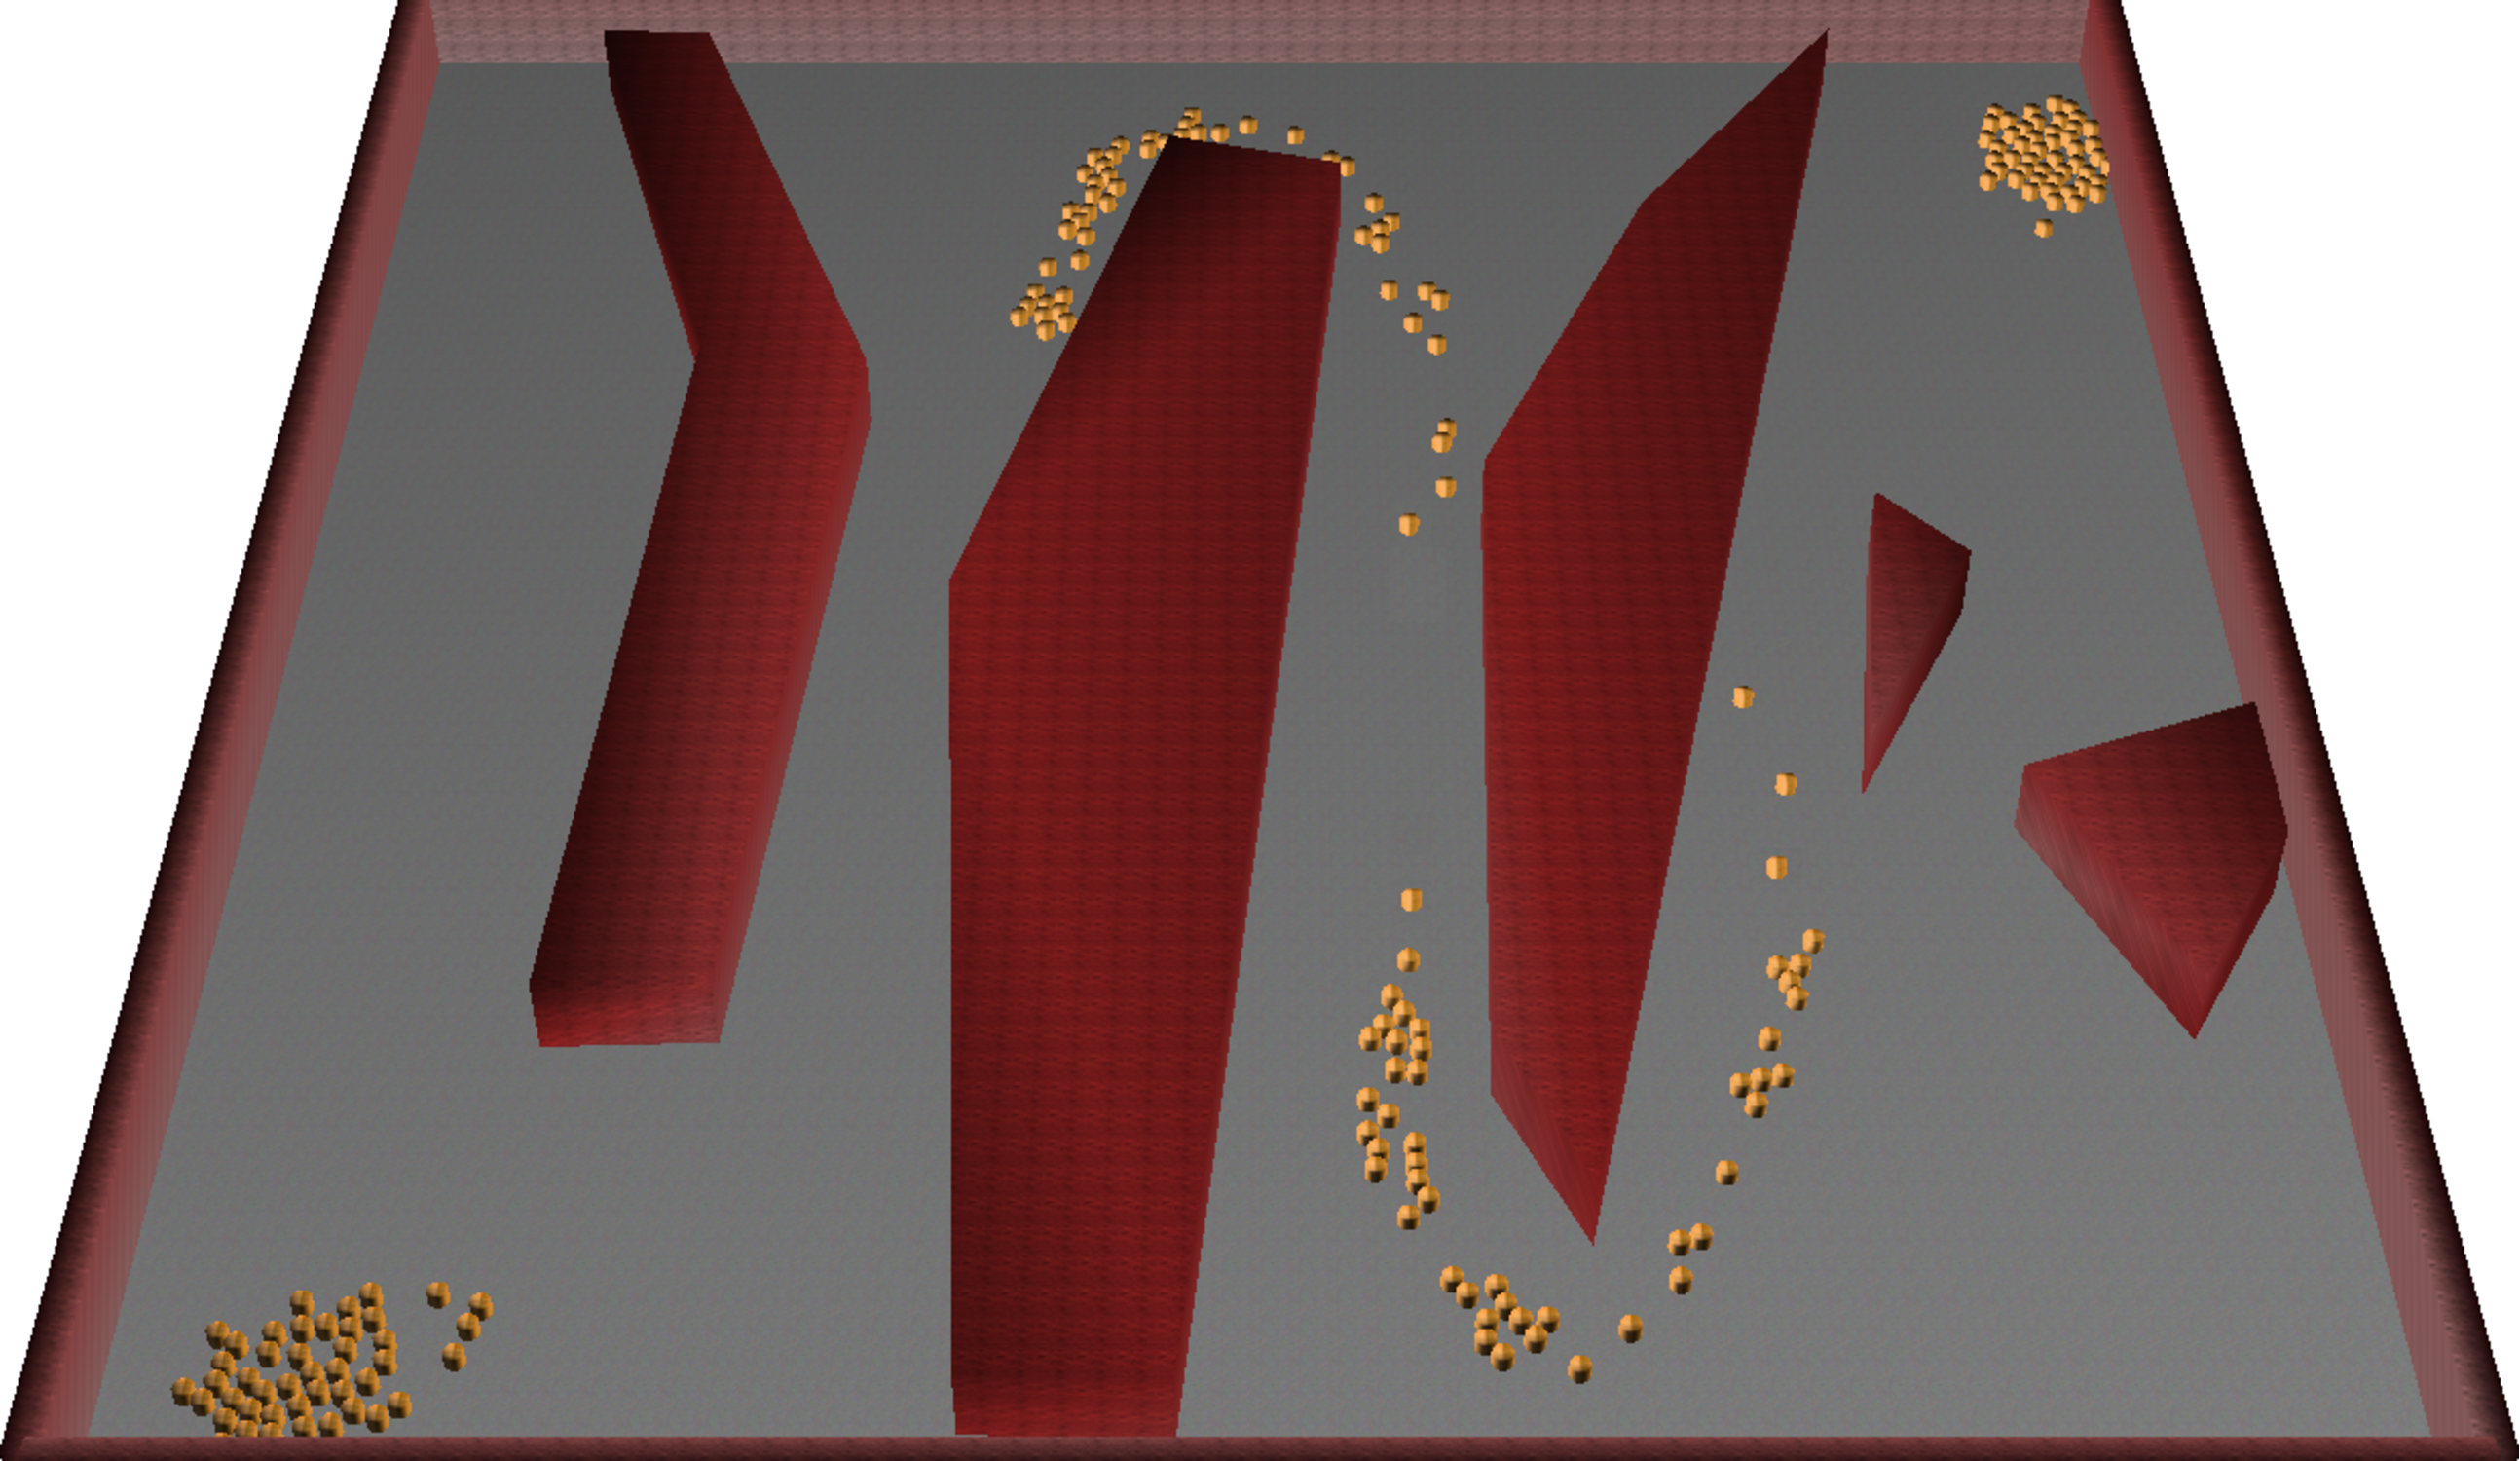
\includegraphics[width=0.55\textwidth]{figs/m7}&
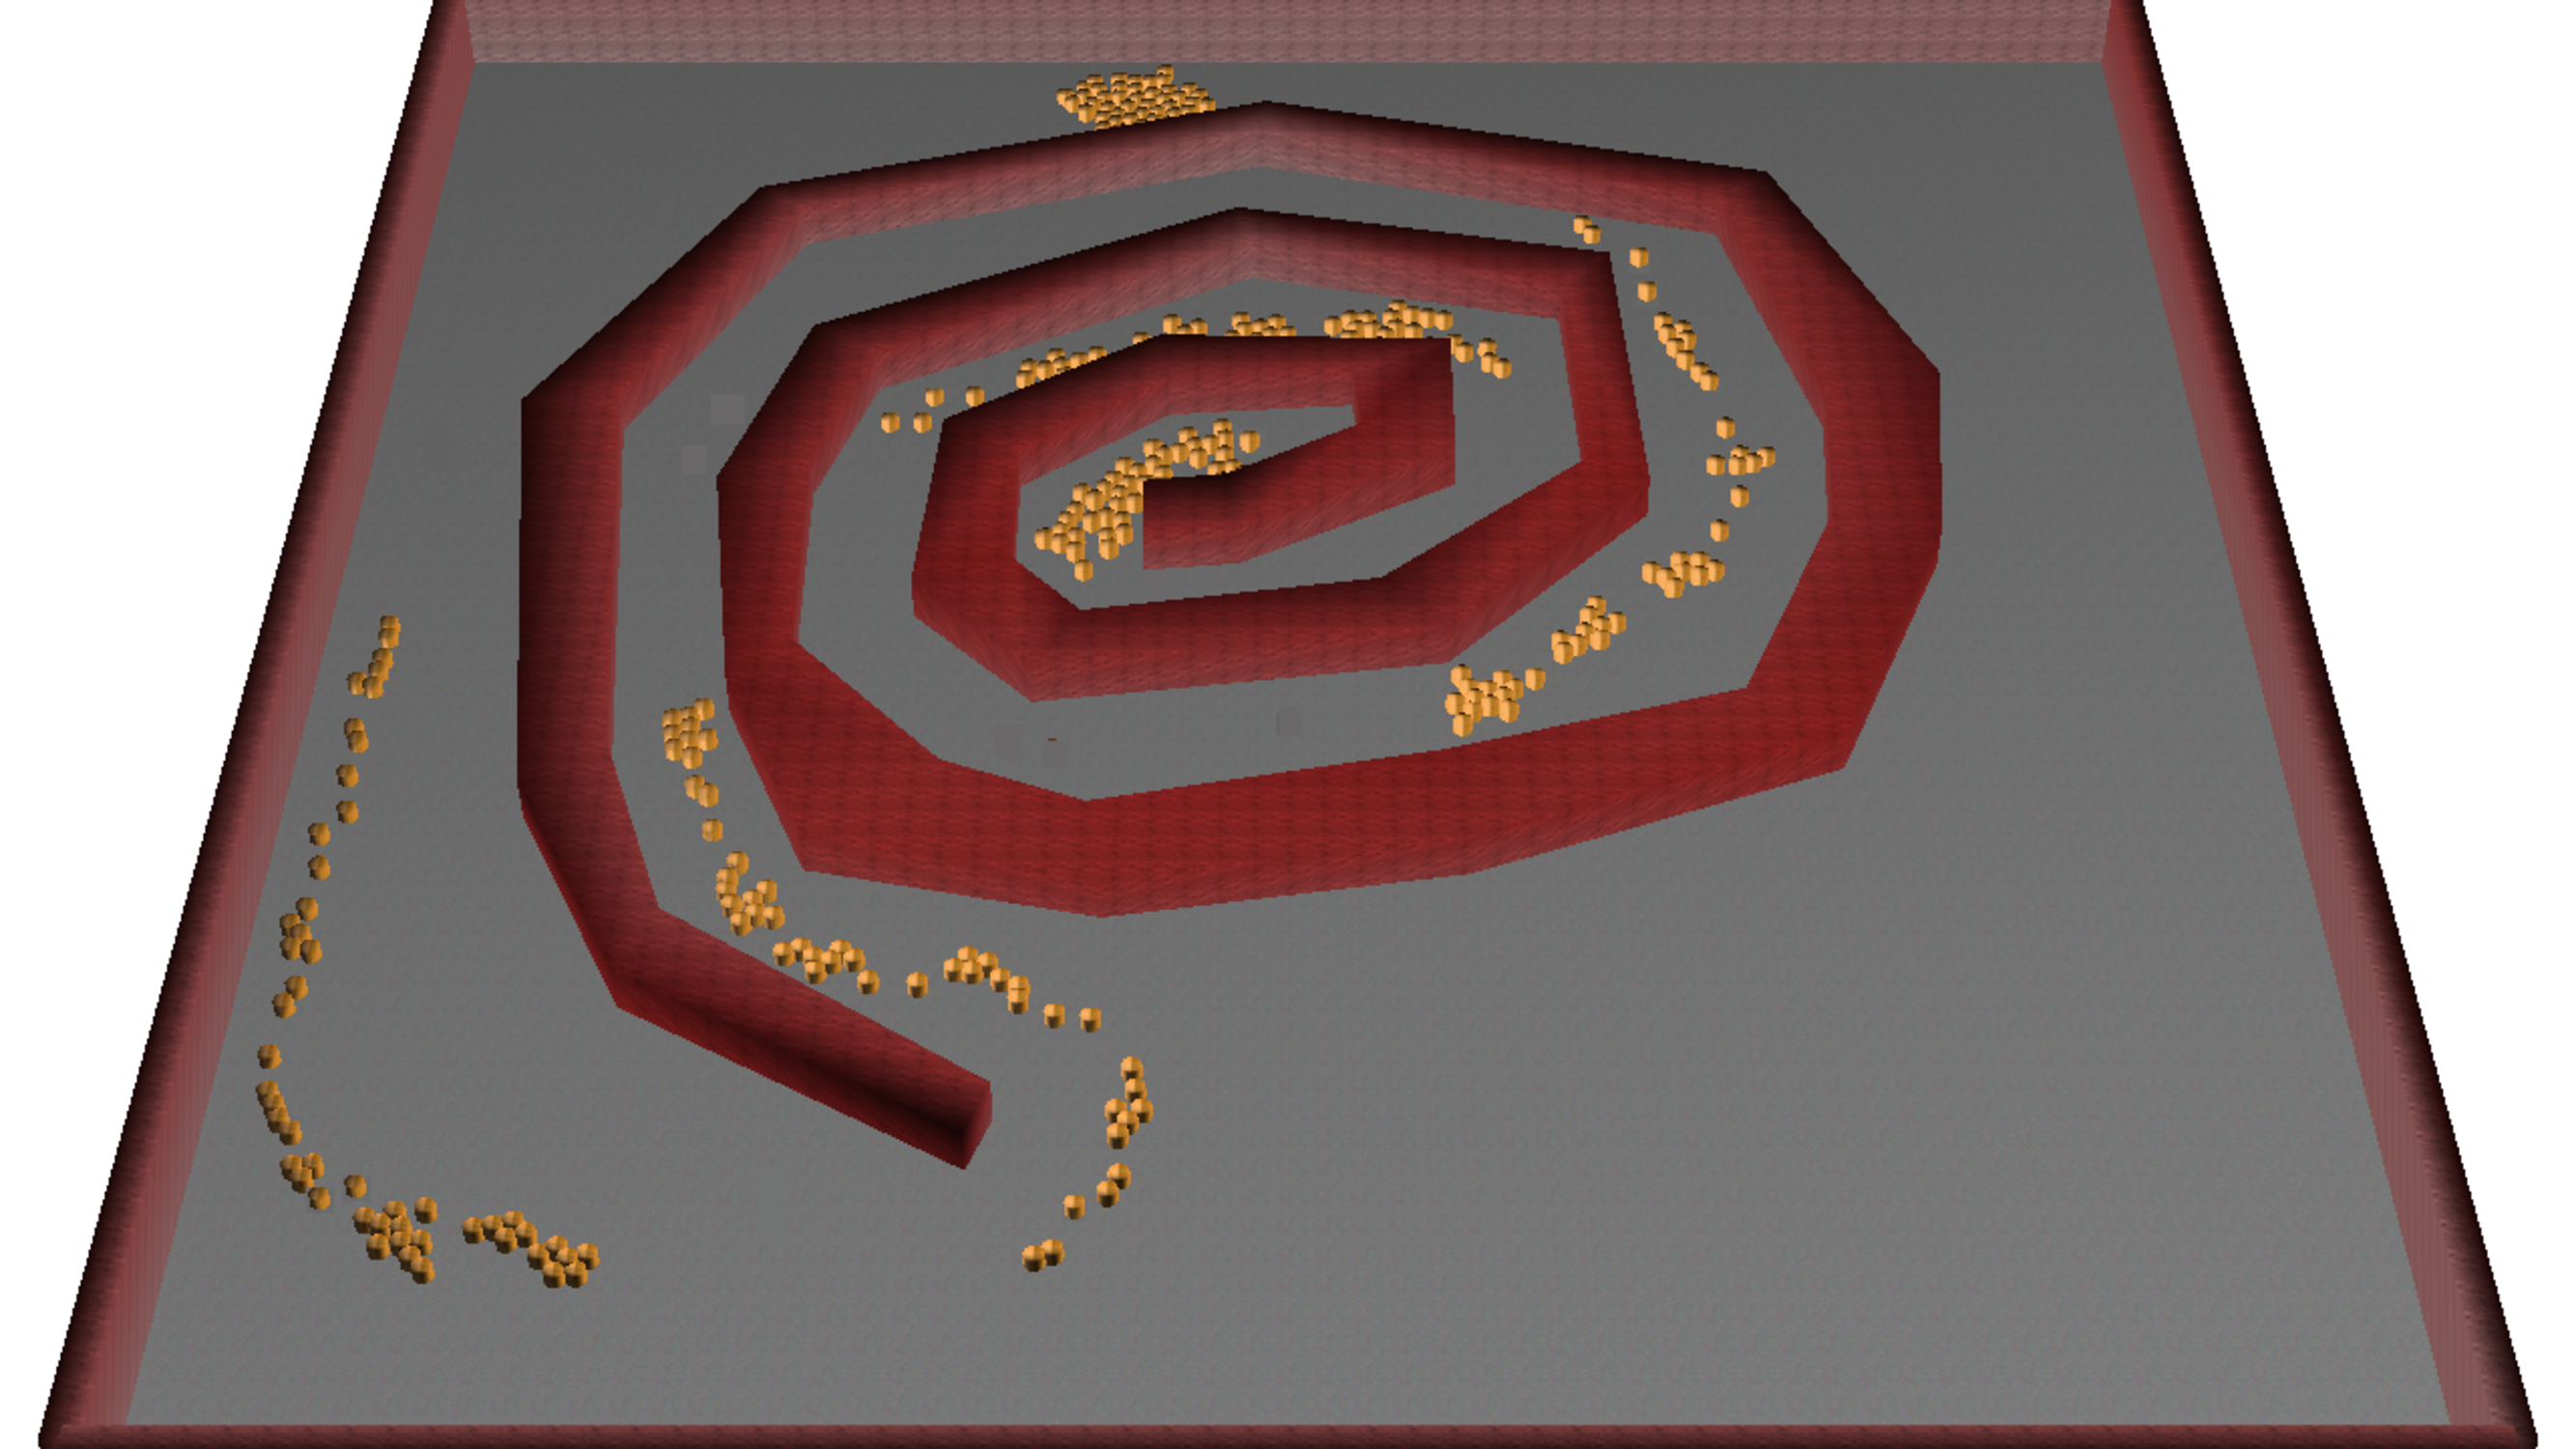
\includegraphics[width=0.55\textwidth]{figs/scene1}\\
(a) scene1 & (b) scene2\\
\multicolumn{2}{c}{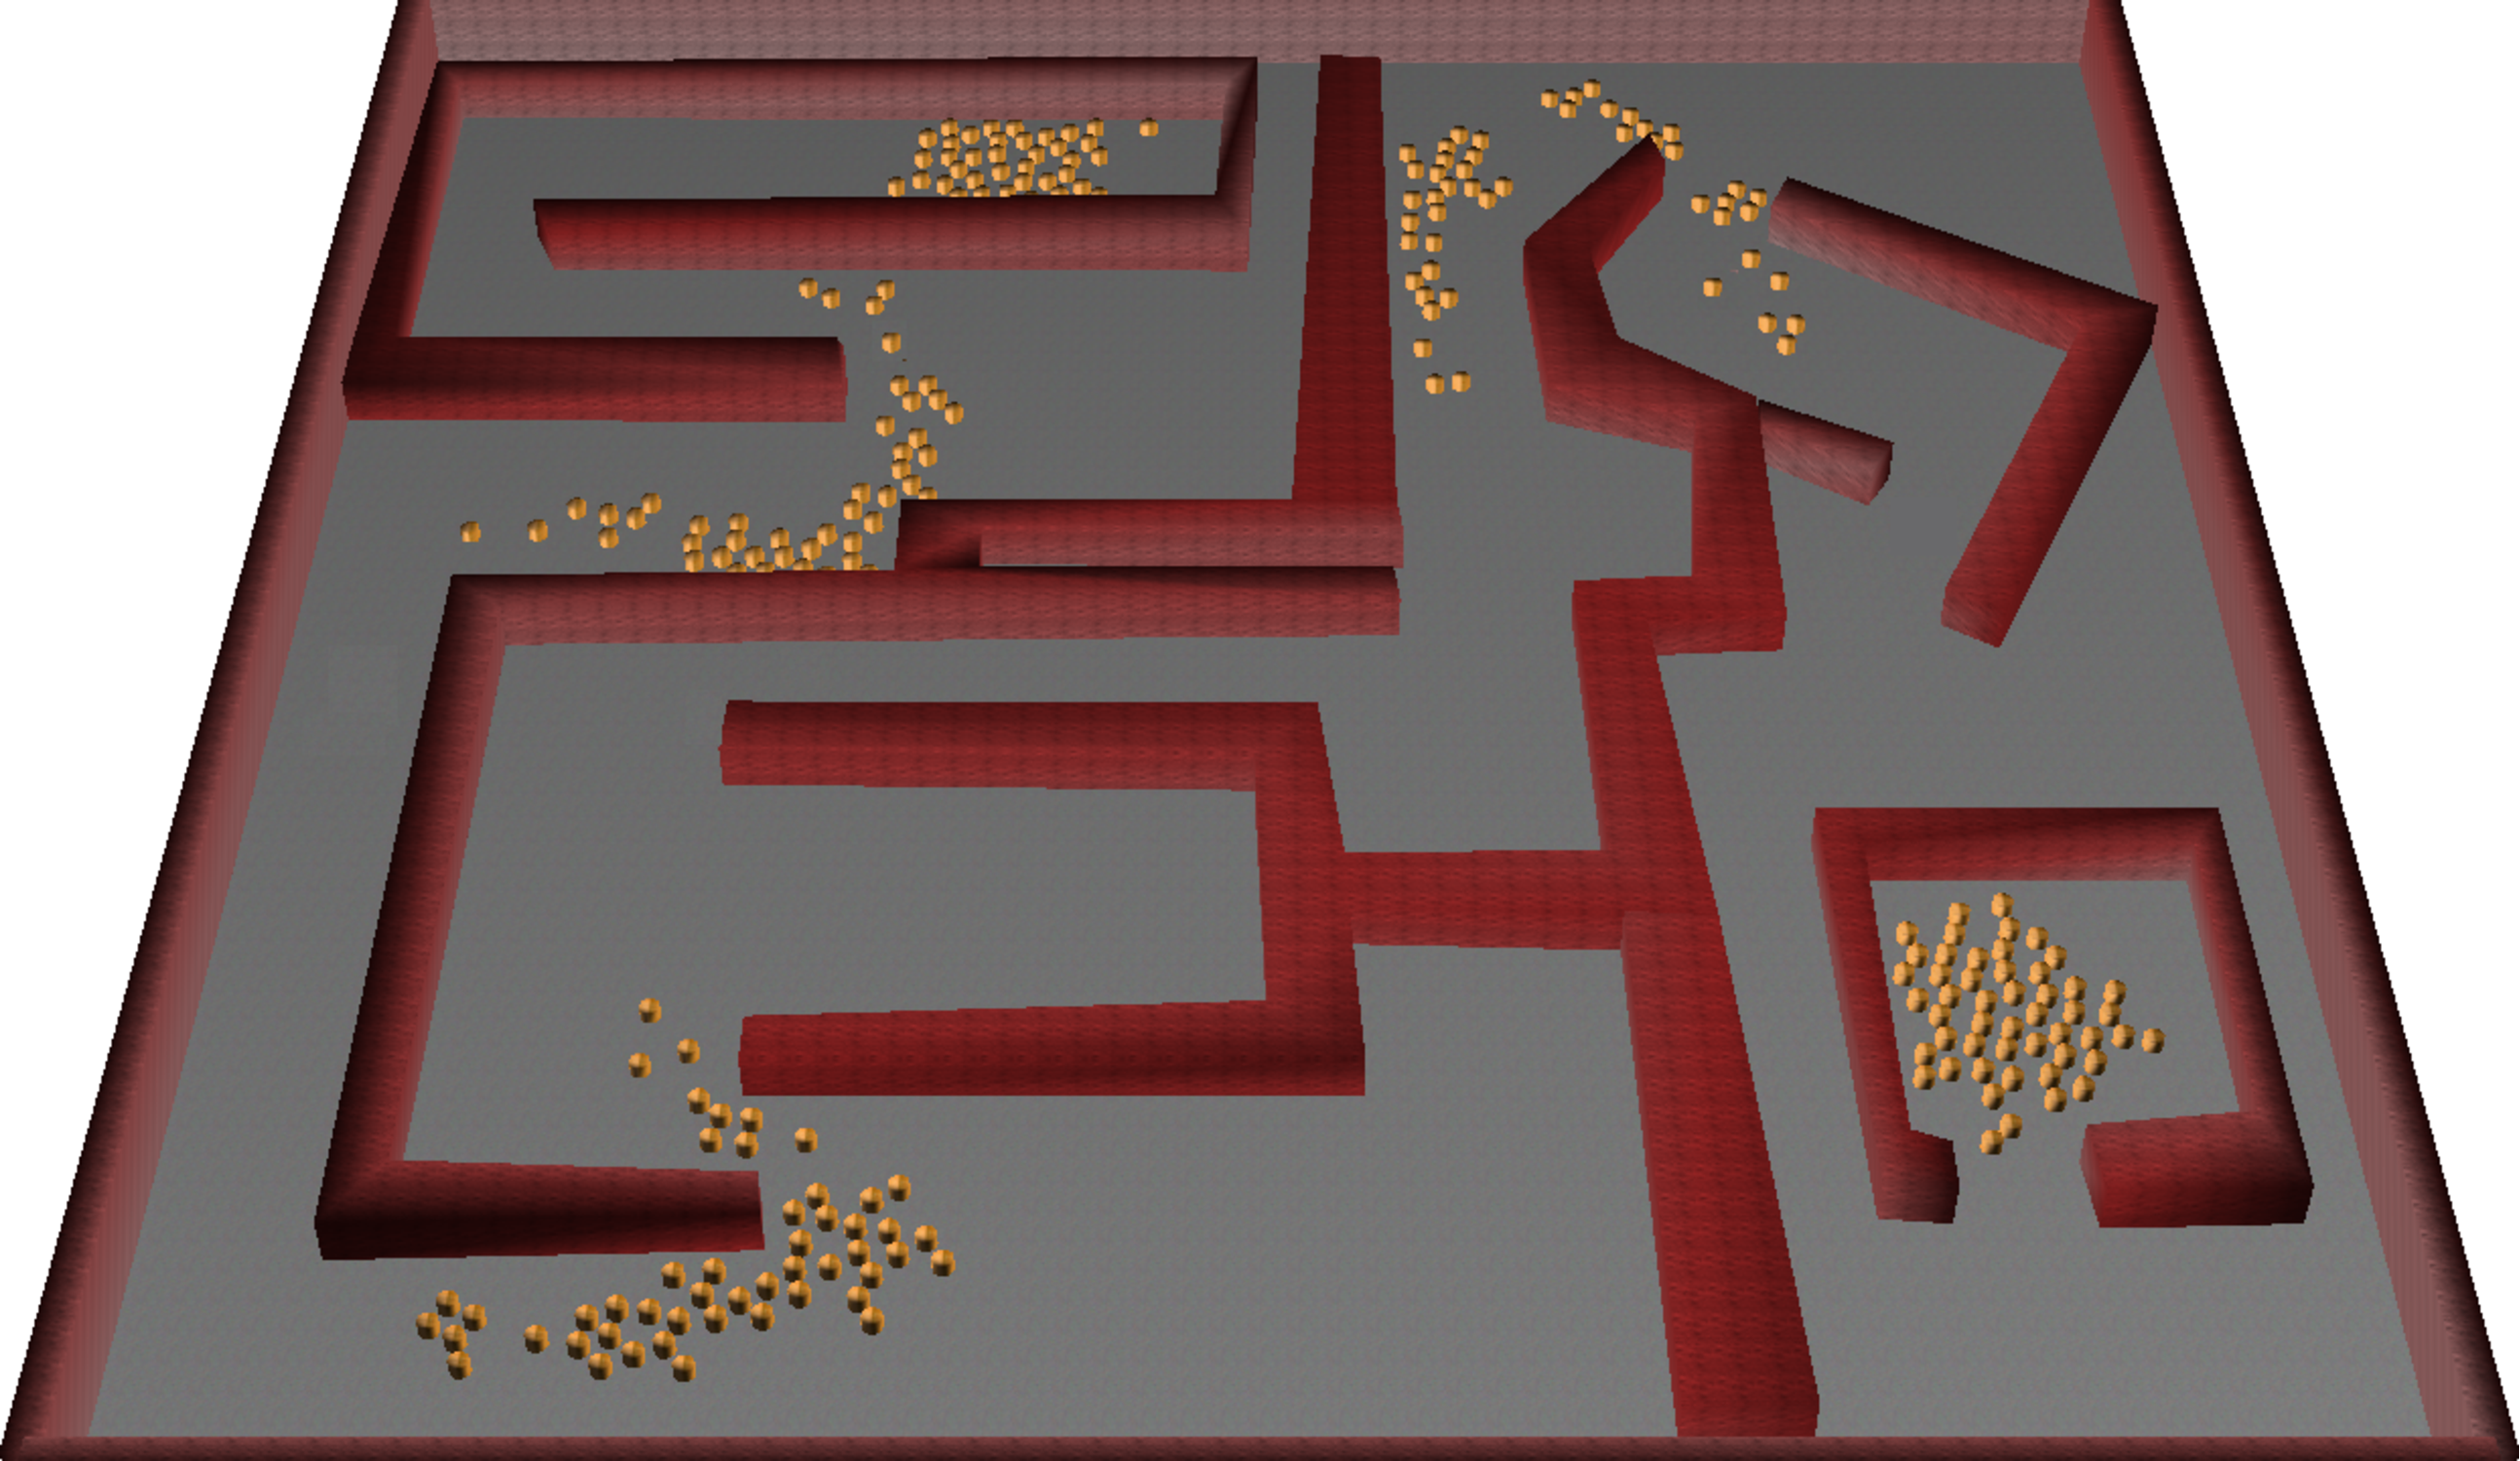
\includegraphics[width=0.55\textwidth]{figs/scene2}}\\
\multicolumn{2}{c}{(c) scene3}
\end{tabular}
\caption{Scenes used in the experiments. Each figure also shows
  intermediate swarm configurations along the path from the initial to
the goal.} 
\label{fig:Scenes}
\end{figure}

\subsection{Measuring Performance}
\label{sec:Measures}
A problem instance is defined by a scene and the number of robots. Due
to the probabilistic nature of the roadmap, performance on a
particular problem instance is based on twenty different runs.
Results report the average time for all the robots to reach the final
destination. Results also report the average distance among all the
robot pairs. More specifically, the average distance for a problem instance is measured by
adding all the pairwise distances at every time step for all the runs
to a vector and then diving by the size of the vector. Finally, the
average distance is scaled by the robot diameter. As an example, a
scaled distance of $5.14$ indicates that the swarm is maintaining an average
separation distance of roughly $5$ robots.  Small values (close to $1$)
indicate that the robots are too close to one another and large values
indicate that the robots are separating. Standard deviations are shown
for both time and scaled distance results.

%$$
%\sum_{run=1}^{20}\sum_{t}
%\left(\sum_{\stackrel{b_i, b_j \in \Var{Robots}}{b_i \neq b_j}}
%||\Var{pos}_t(b_i), \Var{pos}_t(b_j)||_2\right)
%$$

Experiments are conducted on an Intel Core i3 machine (CPU: 2.40GHz,
RAM: 4GB) using Ubuntu 13.04. Code is written in Python 2.7.3. Code is
publicly available at \cite{CodeBoids}.

\subsection{Results}
\label{sec:Results}

Fig.~\ref{fig:ResT}(a) provides a summary of the results on the
average time for all the robots to reach the final
destination. These results indicate that $\Name$ is capable of
effectively planning motions for large swarms moving through
complicated environments. Fig.~\ref{fig:ResT}(b) takes a closer
look at these results by showing how
the average time scales as a function of the number of robots in the
swarm. As the results indicate, the time grows only linearly. Such
results provide promising validation on the scalability of $\Name$. 

\begin{figure}
\centering
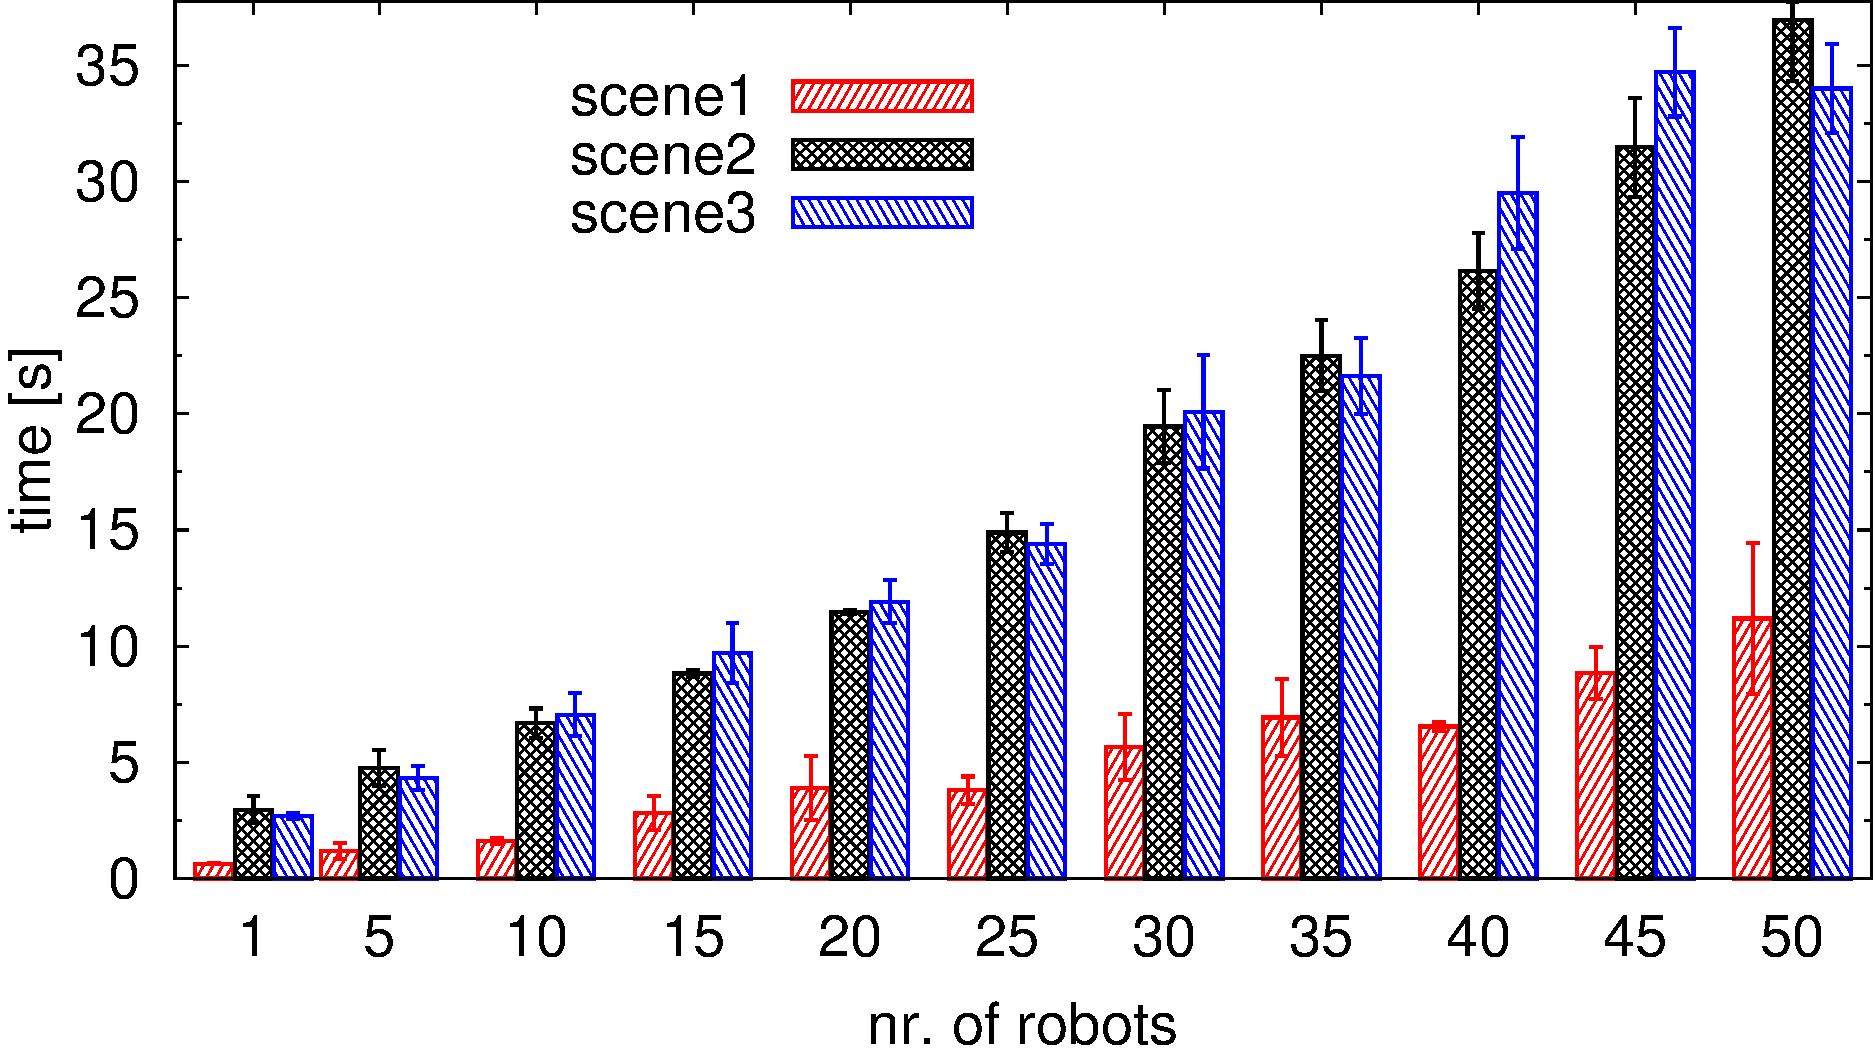
\includegraphics[width=0.49\textwidth]{figs/figResT}
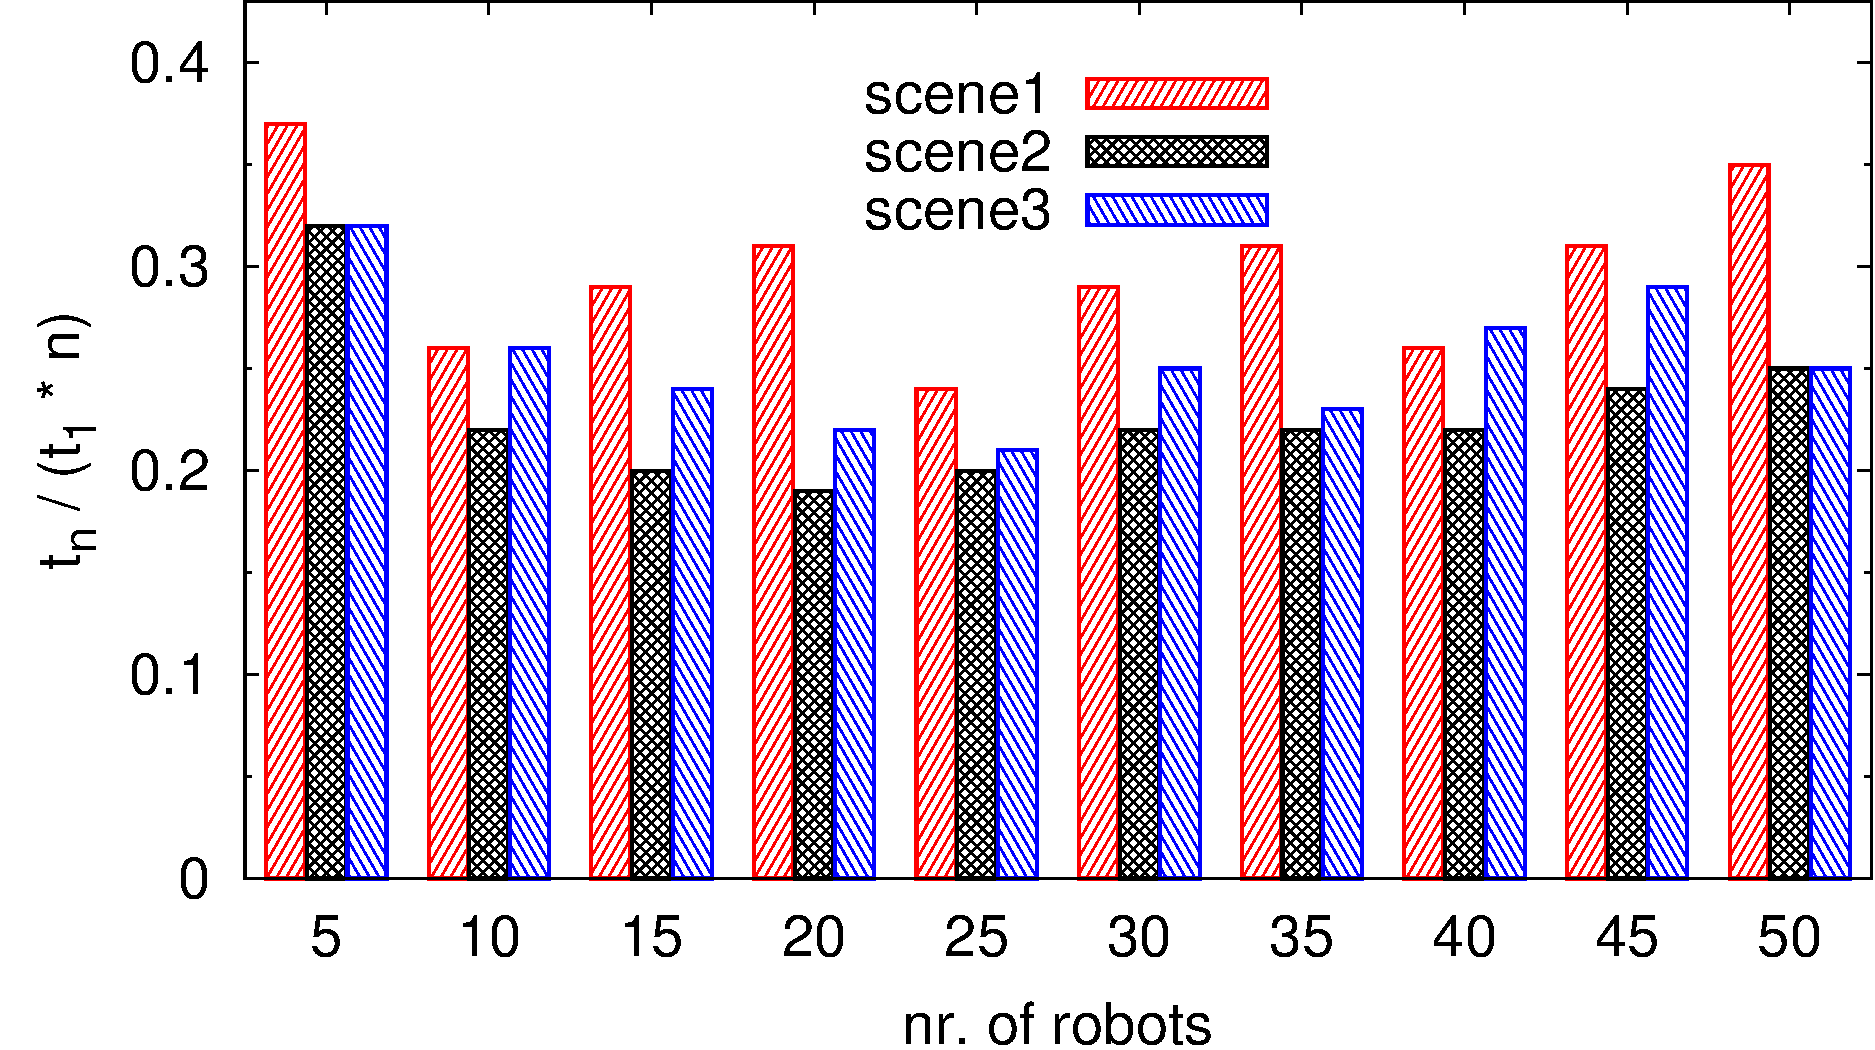
\includegraphics[width=0.49\textwidth]{figs/figResST}
\caption{(a) Results on the average time for all the robots to reach the
  final destination as a function of the number of robots. Bars
  indicate one standard deviation. (b) Scaled results, where $t_n$
  denotes the average time for all $n$ robots to reach the final destination.}
\label{fig:ResT}
\end{figure}

\noindent
The efficiency of $\Name$ derives from the combination of global path
planning via probabilistic roadmaps with local path planning via
potential fields.  To test this further, $\Name$ was run without the
probabilistic roadmap. In this scenario, the robots would be guided by
the potential fields and only be attracted to the final destination
but not to any intermediate goals. Without probabilistic roadmaps,
however, the approach timed out and failed to send any robot to the
final destination. These experiments indicate the importance of
combining probabilistic roadmaps with potential fields when planning
motions for large swarms in complicated environments.


Fig.~\ref{fig:ResFL} shows the average time difference between the
first and the last robot to reach the final destination. The plot
shows that the robots reach the final destination nearly at the same
time even as the number of robots is increased. These results indicate
that the robots remain together and move as a swarm.  



\begin{figure}
\centering
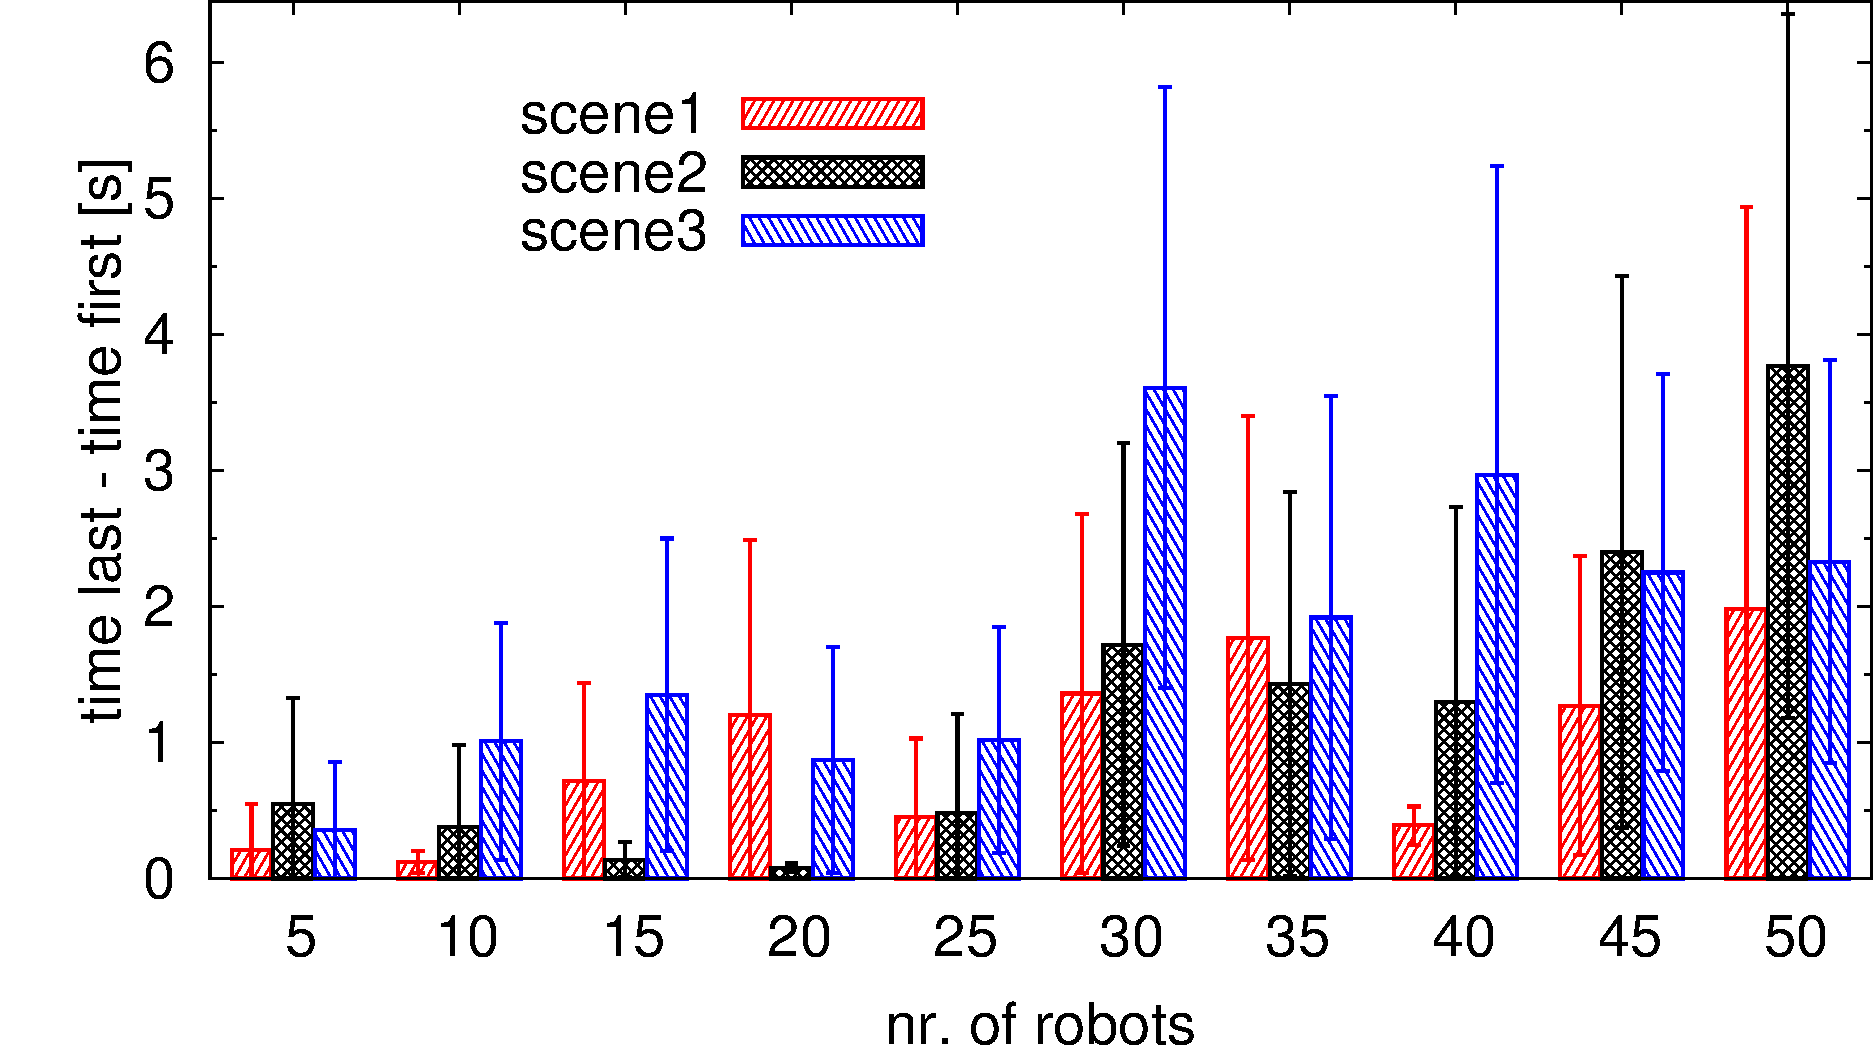
\includegraphics[width=0.65\textwidth]{figs/figResFL}
\caption{Results on the average time difference between the first and
  the last robot to reach the
  final destination as a function of the number of robots. Bars
  indicate one standard deviation.}
\label{fig:ResFL}
\end{figure}

Fig.~\ref{fig:ResD} shows the average scaled distance among all robot
pairs (see Section~\ref{sec:Measures}). The scaled distance provides
an indication of how close the robots are to one another. It is
desirable that the robots are neither too close (as it could cause
collisions or getting stuck in local minima) nor too far from each
other (as it could cause some robots to get separated from the
swarm). The results indicate that the robots maintain a desirable
separation distance. Moreover, the separation distance changes very
little even as the number of robots is increased.

\begin{figure}
\centering
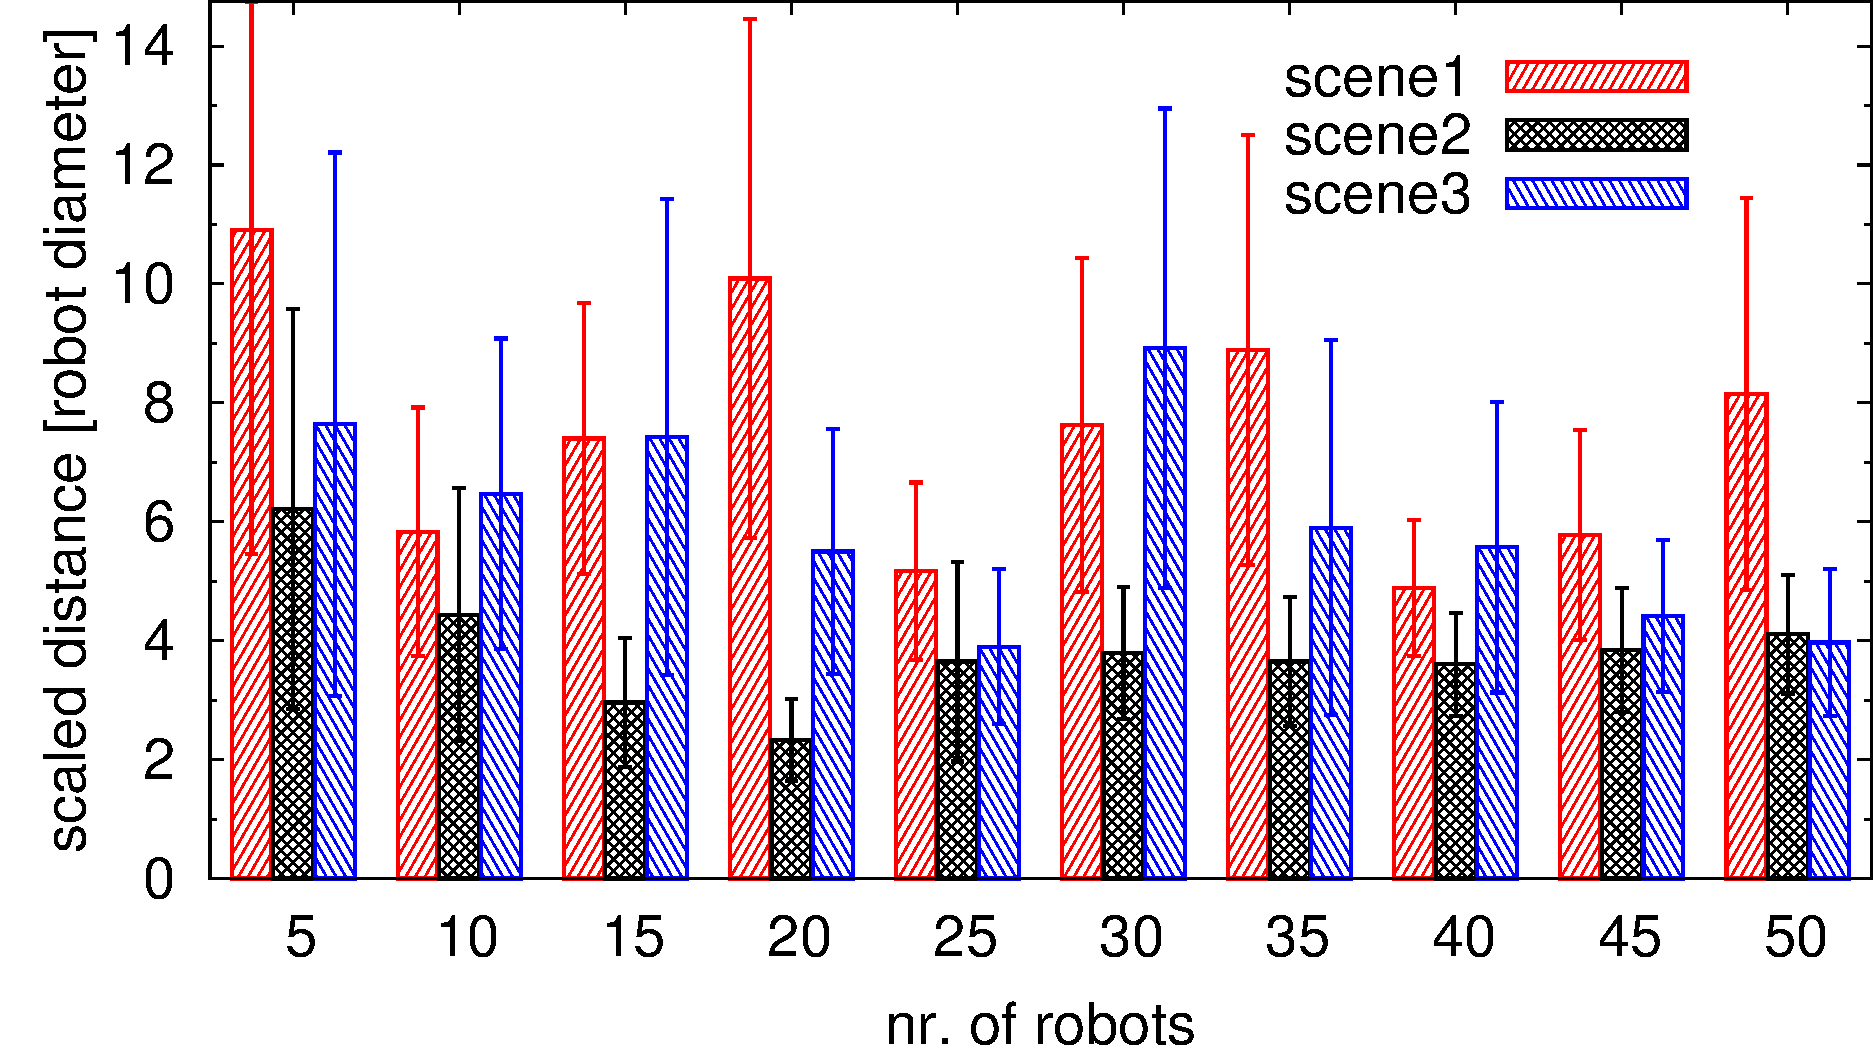
\includegraphics[width=0.65\textwidth]{figs/figResD}
\caption{Results on the average scaled distance among all robot pairs
  as a function of the number of robots. Scaling is done with respect
  to the robot diameter. Bars
  indicate one standard deviation.}
\label{fig:ResD}
\end{figure}


\section{Discussion}

The proposed approach, $\Name$, combined probabilistic roadmaps with
APFs in order to enable a swarm of robots to effectively move to a
desired destination while avoiding collisions with obstacles and each
other.  The probabilistic roadmap provides global path planning to
determine appropriate intermediate goals for the swarm. The potential
fields provide local planning to enable the robots move together as a
swarm towards the goal while avoiding collisions.

The combination of probabilistic roadmaps with APFs opens up several
venues for future research. One research direction is to improve the
interplay between the roadmap planning and APFs in order to more
effectively move the swarm to the desired destination. Another
research direction is to accommodate moving obstacles. As the motion
direction and velocity of the moving obstacles might not be known in
advance, it will be important to be able to predict such motions
and take them into account during planning.

\bibliographystyle{IEEEtran} 
\bibliography{mp,plaku}


\end{document}

